% id: 183-09
% book: 개념원리 중학 3-1 · 19 이차함수 (3)
% section: 중단원 마무리하기 STEP 1 기본 문제
% figure: crop:fig-183-09.png
% answer: ④
% answer_source: 답지
% variant_level: 0 (원본 전사)
% 이 파일은 build.mjs 가 items.json 에서 만든다. 고칠 때는 items.json 을 고친다.
\smash{\raisebox{3.5mm}{\dmkichul{개념원리 중학 3-1 183쪽 09번}}}
다음 중 이차함수 $y=-\dfrac{1}{3}(x-2)^2-1$의 그래프로 알맞은 것은?
\par\smallskip\begin{center}\setlength{\dmfigw}{186.4pt}\ifdim\dmfigw>\linewidth\setlength{\dmfigw}{\linewidth}\fi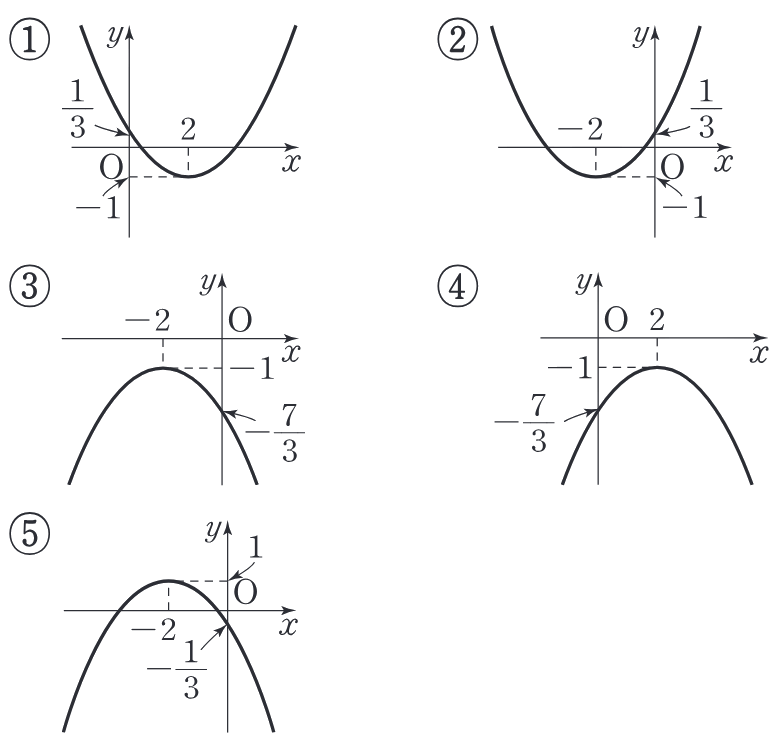
\includegraphics[width=\dmfigw]{figures/fig-183-09.png}\end{center}
